\def\DoNotLoadEpstopdf{}
\documentclass[tikz,border=4pt]{standalone}
% Shared style for the technical appendix figures (2026-10-26).
% Builds on the proposal's figstyle.tex (same fonts, colors, and box styles) and adds
% one encoding for development status, used the same way in every appendix figure.
%   built and tested   solid border (the proposal's normal box styles)
%   built, no test     solid border, and the box text says "no test"
%   specified          dashed border            -> add the key  spec
%   planned            dotted grey border        -> use the style planned
%   no code (by hand)  dotted arrow              -> add the key  byhand
%   outside the artifact  solid grey border      -> use the style outside
% Shared style for proposal figures (2026-10-22 visuals pass).
% Sized to print at 6.5 in (16.5 cm) wide; body text 9 pt sans, nothing below 8 pt.
\usepackage[T1]{fontenc}
\usepackage[scaled=0.95]{helvet}
\renewcommand{\familydefault}{\sfdefault}
\usepackage{xcolor}
\usetikzlibrary{arrows.meta,positioning,calc,patterns.meta}
\definecolor{cink}{HTML}{16191F}
\definecolor{cmuted}{HTML}{4B5563}
\definecolor{cslate}{HTML}{2F4858}
\definecolor{cslatefill}{HTML}{E9EFF3}
\definecolor{cbrass}{HTML}{7A5C12}
\definecolor{cbrassfill}{HTML}{F5EFDE}
\definecolor{cred}{HTML}{8C2F39}
\definecolor{credfill}{HTML}{F8E9EA}
\definecolor{cgreen}{HTML}{235C53}
\definecolor{cgreenfill}{HTML}{E3F0EC}
\definecolor{caudit}{HTML}{5B3A8E}
\definecolor{cauditfill}{HTML}{EFE9F6}
\definecolor{cghost}{HTML}{6B7280}
\definecolor{cghostfill}{HTML}{F3F4F6}
\tikzset{
  >={Triangle[length=5pt,width=4.5pt]},
  box/.style={draw, rounded corners=1.5pt, line width=0.8pt, align=center, inner sep=4pt, font=\fontsize{9}{11}\selectfont},
  sub/.style={font=\fontsize{8}{9.6}\selectfont, text=cmuted},
  ai/.style={box, draw=cbrass, fill=cbrassfill, text=cbrass},
  ver/.style={box, draw=cred, fill=credfill, text=cred},
  pipe/.style={box, draw=cslate, fill=cslatefill, text=cslate},
  prod/.style={box, draw=cslate, fill=cslate, text=white},
  person/.style={box, draw=cink, fill=white, text=cink},
  ghost/.style={box, draw=cghost, fill=cghostfill, text=cghost, dash pattern=on 3pt off 2pt},
  flow/.style={->, line width=0.8pt},
}

\renewcommand{\ttdefault}{lmtt}% vector typewriter font (same design as the default, not a bitmap)
\tikzset{
  spec/.style={dash pattern=on 3pt off 2pt},
  planned/.style={box, draw=cghost, fill=cghostfill, text=cghost, dash pattern=on 0.9pt off 1.6pt},
  outside/.style={box, draw=cghost, fill=white, text=cghost},
  byhand/.style={dash pattern=on 0.9pt off 1.6pt},
  prog/.style={font=\fontsize{8}{9.6}\selectfont\ttfamily},
  legendbox/.style={draw, rounded corners=1pt, line width=0.8pt, minimum width=0.55cm, minimum height=0.32cm, inner sep=0pt},
  legendtext/.style={font=\fontsize{8}{9.6}\selectfont, text=cink, anchor=west, inner sep=1pt},
}
% \statuslegend{x}{y} draws the four-item status legend with its left edge at (x,y).
\newcommand{\statuslegend}[2]{%
  \begin{scope}[shift={(#1,#2)}]
    \node[legendbox, draw=cink, fill=white] (lg1) at (0.275,0) {};
    \node[legendtext] at (0.65,0) {Built and tested};
    \node[legendbox, draw=cink, fill=white, spec] (lg2) at (3.35,0) {};
    \node[legendtext] at (3.725,0) {Specified};
    \node[legendbox, draw=cghost, fill=cghostfill, dash pattern=on 0.9pt off 1.6pt] (lg3) at (5.75,0) {};
    \node[legendtext] at (6.125,0) {Planned};
    \node[legendbox, draw=cghost, fill=white] (lg4) at (7.85,0) {};
    \node[legendtext] at (8.225,0) {Outside the research artifact};
  \end{scope}}

% Figure A2 of the 10/26d appendix: how the workflow would connect to the scholar's harness, model,
% and external software through wrappers, MCP servers, and adapters. Design only, no status.
\begin{document}
\hyphenpenalty=10000
\frenchspacing
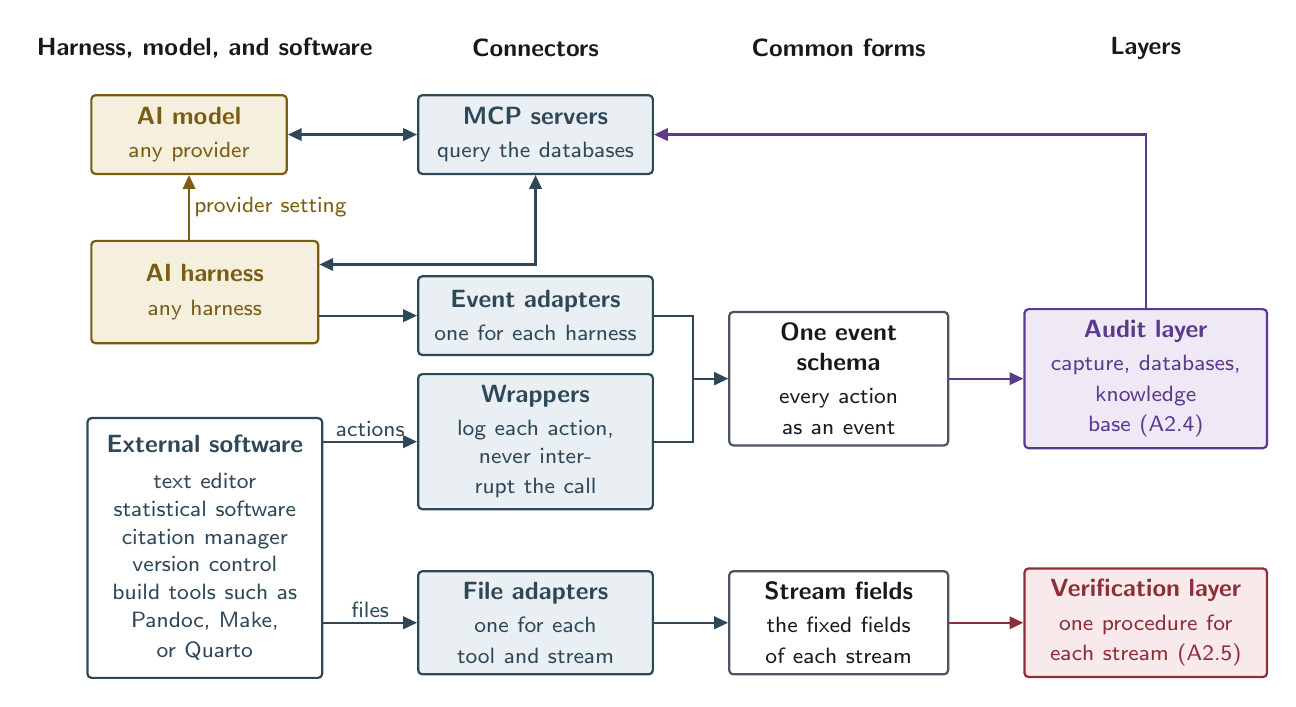
\begin{tikzpicture}
\tikzset{
  col/.style={font=\fontsize{9}{11}\selectfont\bfseries, text=cink},
  lab/.style={font=\fontsize{8}{9.4}\selectfont, inner sep=1.5pt},
  ext/.style={box, draw=cslate, fill=white, text=cslate},
  form/.style={box, draw=cmuted, fill=white, text=cink},
  aud/.style={box, draw=caudit, fill=cauditfill, text=caudit},
}
\newcommand{\sm}[1]{{\fontsize{8}{9.4}\selectfont #1}}
\newcommand{\hd}[1]{{\fontsize{9}{11}\selectfont\bfseries #1}}
% column heads
\node[col] at (1.5,5.0) {Harness, model, and software};
\node[col] at (5.7,5.0) {Connectors};
\node[col] at (9.55,5.0) {Common forms};
\node[col] at (13.45,5.0) {Layers};
% scholar's software
\node[ai, text width=2.2cm, minimum width=2.4cm, minimum height=1.0cm] (mod) at (1.3,3.9) {\hd{AI model}\\[1pt]\sm{any provider}};
\node[ai, text width=2.6cm, minimum width=2.8cm, minimum height=1.3cm] (har) at (1.5,1.9) {\hd{AI harness}\\[1pt]\sm{any harness}};
\node[ext, text width=2.7cm, minimum width=2.9cm, minimum height=3.3cm] (ext) at (1.5,-1.35) {\hd{External software}\\[2pt]\sm{text editor}\\[-1pt]\sm{statistical software}\\[-1pt]\sm{citation manager}\\[-1pt]\sm{version control}\\[-1pt]\sm{build tools such as}\\[-1pt]\sm{Pandoc, Make, or Quarto}};
% connectors
\node[pipe, text width=2.7cm, minimum width=2.9cm, minimum height=1.0cm] (mcp) at (5.7,3.9) {\hd{MCP servers}\\[1pt]\sm{query the databases}};
\node[pipe, text width=2.7cm, minimum width=2.9cm, minimum height=1.0cm] (eva) at (5.7,1.6) {\hd{Event adapters}\\[1pt]\sm{one for each harness}};
\node[pipe, text width=2.7cm, minimum width=2.9cm, minimum height=1.0cm] (wrp) at (5.7,0.0) {\hd{Wrappers}\\[1pt]\sm{log each action,}\\[-1pt]\sm{never interrupt the call}};
\node[pipe, text width=2.7cm, minimum width=2.9cm, minimum height=1.0cm] (fia) at (5.7,-2.3) {\hd{File adapters}\\[1pt]\sm{one for each tool and stream}};
% common forms
\node[form, text width=2.5cm, minimum width=2.7cm, minimum height=1.0cm] (evs) at (9.55,0.8) {\hd{One event schema}\\[1pt]\sm{every action as an event}};
\node[form, text width=2.5cm, minimum width=2.7cm, minimum height=1.0cm] (fld) at (9.55,-2.3) {\hd{Stream fields}\\[1pt]\sm{the fixed fields of each stream}};
% workflow
\node[aud, text width=2.8cm, minimum width=3.0cm, minimum height=1.3cm] (aud) at (13.45,0.8) {\hd{Audit layer}\\[1pt]\sm{capture, databases, knowledge base (A2.4)}};
\node[ver, text width=2.8cm, minimum width=3.0cm, minimum height=1.3cm] (ver) at (13.45,-2.3) {\hd{Verification layer}\\[1pt]\sm{one procedure for each stream (A2.5)}};
% arrows
\draw[flow, cbrass] (har.north -| mod.south) -- node[lab, text=cbrass, right] {provider setting} (mod.south);
\draw[flow, cslate] (har.east |- eva.west) -- (eva.west);
\draw[flow, cslate] (ext.east |- wrp.west) -- node[lab, text=cslate, above] {actions} (wrp.west);
\draw[flow, cslate] (ext.east |- fia.west) -- node[lab, text=cslate, above] {files} (fia.west);
\draw[flow, cslate] (eva.east) -| ($(evs.west)+(-0.45,0)$) -- (evs.west);
\draw[flow, cslate] (wrp.east) -| ($(evs.west)+(-0.45,0)$) -- (evs.west);
\draw[flow, cslate] (fia.east) -- (fld.west);
\draw[flow, caudit] (evs.east) -- (aud.west);
\draw[flow, cred] (fld.east) -- (ver.west);
\draw[flow, caudit] (aud.north) |- (mcp.east);
\draw[<->, line width=0.8pt, cslate] (mcp.south) |- ($(har.east)+(0,0.35)$);
\draw[<->, line width=0.8pt, cslate] (mcp.west |- mod.east) -- (mod.east);
\end{tikzpicture}
\end{document}
